\documentclass[10pt]{article}
\usepackage[polish]{babel}
\usepackage[utf8]{inputenc}
\usepackage[T1]{fontenc}
\usepackage{amsmath}
\usepackage{amsfonts}
\usepackage{amssymb}
\usepackage[version=4]{mhchem}
\usepackage{stmaryrd}
\usepackage{graphicx}
\usepackage[export]{adjustbox}
\graphicspath{ {./images/} }

\title{KLASY PO SZKOLE PODSTAWOWEJ }

\author{}
\date{}


\begin{document}
\maketitle
\begin{enumerate}
  \item Udowodnij, że jeśli \(a\) jest całkowite to liczba \(a^{4}+2 a^{3}-a^{2}-2 a\) jest podzielna przez 24.
  \item Policz długość odcinka \(a\), jeśli wiadomo, że pole gwiazdki wynosi \((3 \sqrt{3}-\pi)\) i jej krawędzie to równe części jednego okręgu.
  \item Połącz wyspy mostami zgodnie z zasadami:
\end{enumerate}

\begin{itemize}
  \item Mosty można przeprowadzić tylko w kierunkach poziomym i pionowym.
  \item Każdy most musi łączyć dwie wyspy.
  \item Mosty nie mogą się przecinać ani nie mogą przechodzić przez wyspy.
  \item Dwie wyspy mogą być połączone między sobą najwyżej dwoma mostami.
\end{itemize}

Liczby na wyspach mówią, ile mostów wychodzi z danej wyspy.\\
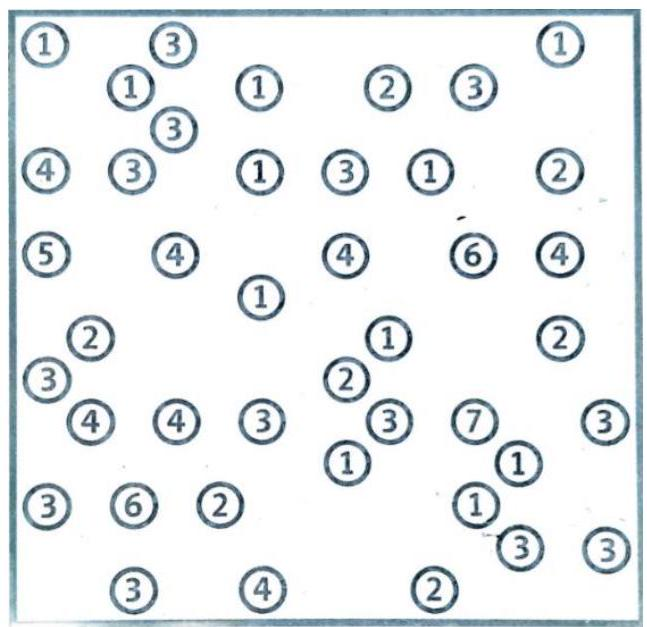
\includegraphics[max width=\textwidth, center]{2024_11_21_583984befecd44b3e998g-1}

\section*{KLASY PO GIMNAZJUM}
\begin{enumerate}
  \item Czworokąt ABCD jest wpisany w okrąg o promieniu R. Punkty KLMN są środkami odpowiednio boków AB, BC, CD i DA. Wykaż, że okręgi opisane na trójkątach AKN, KBL, LCM i MDN są przystające.
  \item Udowodnij, że jeżeli \(a, b, c, d\) są liczbami wymiernymi i \(a+\sqrt{b}=c+\sqrt{d}\) oraz przynajmniej jedna z liczb \(\sqrt{b}, \sqrt{d}\) jest niewymierna, to \(a=c\) i \(b=d\).
  \item Znajdź wszystkie pary liczb wymiernych dodatnich spełniających równanie
\end{enumerate}

\[
\sqrt{a}+\sqrt{b}=\sqrt{106+\sqrt{2020}}
\]


\end{document}